\documentclass[a4paper]{article}
\usepackage{graphicx}

\begin{document}

\section{Introduction}
The billing system codebase is a core component of Acme Telecom's business, and is heavily relied upon by other sections of the code. In the absence of unit and acceptance tests, modifying the codebase becomes a delicate matter, as any modifications may silently break existing functionality. For this reason, we started by building unit and acceptance tests for the existing code, to allow us to validate our work. In some situations, this required the refactoring sections of the code or introduce new technologies to the codebase. \emph{Overall, we have been successful in implementing the necessary extensions, while preserving the APIs and functionality of the original system?}

\subsection{System Design and Division of the Tasks}
For the task we were given access to only part of the code in the com.acmetelecom package. Although it is unclear how much of the code we had not been given access, the lack of a more refined package structure suggests a flat hierarchy in the system, whereby all components have access to all public and package private classes and methods in the system. As such, Throughout the task, we kept the name and signature of such classes and methods for compatibility.

Following our initial analysis of the system as a whole, we decided to start by writing unit tests to validate our changes. Writing these tests was divided up among team members, and we therefore chose to move the codebase to a Git repository for revision control. Following the introduction of several new tools to the system, we additionally added Maven to our project for better control over dependencies.

\section{Unit Testing}
As there were no unit tests for the given code and we wanted to ensure that our final implementation is of a high quality, we wrote unit tests for the existing behaviour. We also followed the {\bf Test Driven Development} techniques and added unit tests for the desired new behaviour and then made them pass by implementing the new features.

While writing unit tests for the existing behaviour we found that some of the existing code is worth refactoring. The following paragraphs describe what cases we have covered with our unit tests and the most important changes we have introduced in each class. While refactoring we ensured that no public APIs are changed so that no components from other departments depending on our billing system could be broken.

\subsection{DaytimePeakPeriod.java}

{\bf Unit tests:} We check whether a given time is correctly classified to either a peak or an off-peak time.
\\{\bf Refactoring:} We added a new constructor of the class that takes a peak start and end hour as parameters to make the testing easier. We also introduced a default constructor and default peak start and end hours to mimic the original behaviour.

\subsection{MoneyFormatter.java}
{\bf Unit tests:} We test the conversion from pence to pounds with the precision of 2 significant figures. We also make sure that the decimal separator is ‘.’ as we use the UK locale.
\\{\bf Refactoring:} We forced the formatter to use the UK locale, instead of the system default one. As a result the decimal separator would be forced to the UK ‘.’ instead of ‘,’ on non-UK machines.

\subsection{Call.java, CallStart.java, CallEnd.java}
{\bf Unit tests:} We test whether all the details of a call are correct after initialising a Call object (Callee, duration of the call, date, start and end time).
\\{\bf Refactoring:} We forced the use of the UK locale in Call.java to ensure that the date is formatted in the same way across all the systems. We also added a timestamp parameter to the constructors in CallStart.java and CallEnd.java. At the same time, we made the old constructors call with timestamp = System.currentTimeMillis() to preserve the old behaviour.

\subsection{CallEvent.java}
{\bf Unit tests:} We assert that the correct caller, callee and time are used.
\\{\bf Refactoring:} We added an abstract copy() method (implemented in CallStart.java and CallStart.java) used to safely return the last CallEvent from the BillingSystem. This ensures that in case a user decides to modify the instance that was passed on to him it will not modify the instance stored in the billing system.

\subsection{BillingSystem.java}
{\bf Unit tests:} We used Mockito to create mock CustomerDatabase and TariffLibrary objects. We then test whether all the details of a call that has been initiated are correct, e.g. we verify the number of calls for a given customer or check that we call our functions a correct number of times. We also added a CustomerMatcher Hamcrest ArgumentMatcher implementation that is used with Cucumber to compare the customers field by field.
\\{\bf Refactoring:} We added a new constructor that takes CustomerDatabase, TariffLibrary and BillGeneratorFactory parameters. This change decouples the BillingSystem class from concrete implementations of said parameters. This change is described in more detail in section 3.

\subsection{HtmlPrinter.java}
{\bf Unit tests:} As the methods in HtmlPrinter print part of the bill as HTML to the standard output some code had to be written to capture the output and test it. We used {\bf JTidy} to parse the output and check for errors. We also unit tested the methods printing each part of the bill and the new method printing the whole bill.
\\{\bf Refactoring:} Printing to the standard output is an example of a bad design. Other ways of printing should have been made available, e.g. printing to a file that could then be sent over email. As the existing methods allowed only for printing part of the bills we added a new method that generates an entire bill. This is good for extensibility, since other printer types might assemble a bill differently.

The methods have been refactored so that they do not open HTML tags without closing them making the code more robust. The old methods are still available to be used since they were part of the public API and might be used by the other components that we do not know about. They have been marked as deprecated to discourage their use. 

\subsection{BillGenerator.java}
{\bf Unit tests:} We generate a test bill and check if the correct bill is printed to the standard output.
\\{\bf Refactoring:} The old BillGenerator called different methods to assemble the bills. We introduced a much simpler solution that requires the generator to just pass the parameters to the printBill function of the HtmlPrinter and deprecates the old constructor.







\section{Acceptace tests}
In order to improve the communication between the developers and the management and ensure their requirements for this project are met, we introduced acceptance tests. Our system follows a {\bf Ports-and-Adapters} architecture, so our acceptance tests can run directly against the domain model classes.

After evaluating several tools, we chose {\bf Cucumber}, a software that tries to bridge the gap between specifications and acceptance tests. It allows us to represent a specification in the form of scenarios written in plain language that can be later executed and verified. The main advantage of this choice is that writing the specifications is extremely easy, it requires no developer knowledge and the instrumentation can be done directly on the Java code via annotations. On the other side, we found it difficult to work with at the beginning due to the poor documentation, but once becoming familiar with the API, it made our job a lot easier.

In order to decouple our acceptance tests we mocked the customers and tariff databases using {\bf Mockito} testing framework, e.g.:

\begin{figure}[h]
\begin{verbatim}
Mockito.when(tariffsDb.tarriffFor(Mockito.argThat(
new PlanMatcher(customer)))).thenReturn(Tariff.valueOf(pricePlan));
\end{verbatim}
\caption{Example of using mock objects in our code.}
\end{figure}

We also decided to use the {\bf Joda Time} as we found it much simpler and clearer than its java.util equivalents used in the existing implementation of the project.

Our workflow for executing given scenarios looked as follows:
\begin{enumerate}
\item Write the specification steps in plain text using a DSL called {\bf Gherkin}, e.g.:

\begin{figure}[h]
\begin{verbatim}
Scenario: Peak-Peak
    When 001 calls 002 at "25/10/13 15:00:00"
    And 001 ends call with 002 at "25/10/13 18:14:00"

    Then the bill for Alan with number 001 and plan Standard shows:
        |     Time        | Number      | Duration  | Cost    |
        |25/10/13 15:00   | 002         | 194:00    | 5820    |
    And total 5820

\end{verbatim}
\caption{Example Cucumber scenario.}
\end{figure}

Every step puts the application in a different state, so one scenario can influence the outcome of another. We used the background definition to create an unnamed scenario (setting up the customer database) to ensure that the application gets in a known state before executing any other scenarios:

\begin{figure}[h]
\begin{verbatim}
Scenario: Peak-Peak
   Background:
      Given the following customer database:
          |   FullName  | PhoneNumber | PricePlan |
          | Alan        |     001     | Standard  |
          | Steve       |     002     | Standard  |

\end{verbatim}
\caption{Example use of background in our code.}
\end{figure}

\item Link the steps to the step definitions.
\item Verify the specified behaviour with the application under test.
The following code is used to run the Cucumber tests:

\begin{figure}[h]
\begin{verbatim}
@RunWith(Cucumber.class)
@Cucumber.Options(features = "src/test/resources",
                  format = {"progress", "html:reports/cucumber"})
public class CucumberTests {
}

\end{verbatim}
\caption{Code for running Cucumber tests.}
\end{figure}

\end{enumerate}

\subsection{Refactoring}
While implementing the acceptance tests, we discovered several weak points in the existing code and decided to refactor sections of the code. Throughout the refactoring process, we made sure to only make minimal changes to the codebase, as refactoring is a risky task that may jeopardize the correctness of the code, specially in the absence of unit/acceptance tests. Moreover, we made sure not to change any existing public APIs, to ensure that any client codebase reliant on the Acme Telecom package would not be affected by our introduction of unit tests. One important exception to this rule, the deprecation of the BillGenerator constructor, is described in more detail below.

One such refactoring made use of the dependency inversion principle to remove hard-coded dependencies from the BillingSystem class. In the original implementation, the BillingSystem class relied upon the CentralCustomerDatabase and CentralTariffDatabase classes, rather than the CustomerDatabase and TariffDatabase interfaces, despite not making any calls outside of the interface methods. This became an issue when writing the acceptance tests, as it meant we were unable to use our own data sets for testing. 

Our solution was to add a novel BillingSystem constructor that would take CustomerDatabase and TariffLibrary objects. This solution preserved the prior, public no-argument constructor, which now simply delegates to our novel constructor using the prior CentralCustomerDatabase and CentralTariffDatabase implementations. Overall, we were successful in exploiting polymorphism, an aspect of object-oriented design, to make the necessary changes to the codebase without modifying any existing functionality.

Another instance of refactoring that enabled us to write acceptance tests was the removal of the BillGenerator constructor calls from the BillingSystem. The BillGenerator class is responsible for sending messages to customers to alert them of any fees due. When testing, it makes sense to mock this class in order to avoid sending out any real bills to customers when testing, however the original BillingSystem had a hard coded dependency to the BillGenerator. Resolving this issue proved more difficult than the previous case, as a new BillGenerator is needed every time a customer was billed, whereas only one instance of the CustomerDatabase and TariffLibrary were needed for a given run of the program. 

We solved this problem by using an abstract factory pattern to delegate creation of the BillGenerator. We felt this was an appropriate choice as only minimal changes were required (the BillGenerator constructor was only used in one location in the entire BillingSystem file), while making it easy for us to inject mocked BillGenerators via a custom factory. As in the previous case, we modified the BillingSystem constructor to take a BillGeneratorFactory as a parameter, while the existing no-argument constructor was altered to make use of the concrete BillGeneratorRealFactory which preserved functionality. One unfortunate downside to our solution was that there were now two ways of instantiating the BillGenerator class, either via the no-argument constructor or the default factory, and we required client code to use our factory exclusively. We therefore decided to mark the constructor as deprecated: this will ask clients to move their code away from the constructor, without breaking any existing functionality in the meantime.

One final instance of refactoring was the overloading of the BillingSystem.callInitiated(...) and the BillingSystem.callEnded(...) methods to take an additional timestamp parameter. Previously, these methods took only the phone numbers associated to a call, with the timestamp computed on the fly according the system clock. This made it difficult to test due to the ever-changing nature of the system time variable. We therefore added callInitiated(...) and callEnded(...) methods that took three parameters, the third being a specific timestamp value. As a consequence, we were also required to introduce CallEvent constructors that would take a timestamp as a parameter. Overall, we were successful in preserving both the existing API and the underlying behaviour while making the necessary changes to enable testing of the code.

\section{Implementation of new features}

The main requirement of the client was to modify the way the customers are charged for the calls made during peak and offpeak periods. As mentioned before, we used a {\bf Test Driven Development} approach, hence all our tests were already implemented by the time we started changing the behaviour. We initially added glue code, so the test went red as the new feature had not been implemented rather than as a result of a lack of glue code. We were then able to focus on the feature implementation, extending the system so that the tests passed. 

In a real life work environment we would meet the client and check with them that our specification documents accurately describe the desired behaviour, but this was not possible for the purpose of this exercise. We considered writing a specification document, but the lecture given by Nat Pryce clearly indicated that such a document would just “hinder learning and continuous improvement”. Instead, we made use of the Cucumber specification steps, previously described in Section 2, which automate the testing and strictly prioritise the features. It constitutes a good documentation for both developers and clients.


\section{Further Added Extensions}

\subsection{Removing Circular Dependencies}

A key takeaway from the course so far has been increasing the maintainability of the code, by reducing coupling or increasing cohesion of classes for example. As in the last coursework, we used the \emph{stan4j} developer tool as well as IntelliJ IDEA's dependency analyser to get a better idea of the structure of the overall architecture.

\begin{figure}[h]
\centering
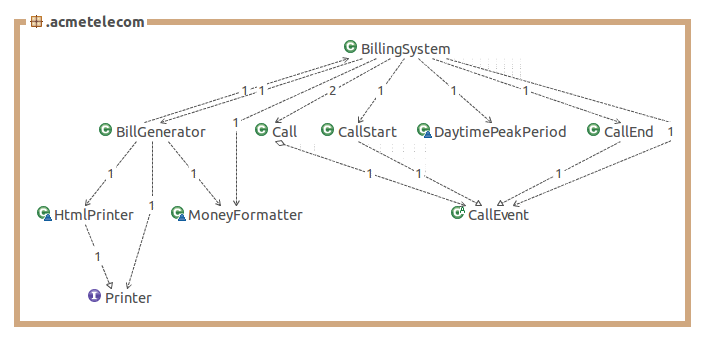
\includegraphics[width=\textwidth]{dependency_graph}
\caption{The dependency graph as indicated by stan4j}
\end{figure}

We observed a circular dependency between BillingSystem and BillingGenerator which could potentially cause issues if we were to replace one of these classes. Our first approach was to remove this dependency by moving LineItem, which is a static inner class of BillingSystem, into its own class. 



\subsection{Maven}

One of the first extensions we implemented in the codebase was porting the project to Maven. A few members of our team had prior experience with creating Maven projects so the process was straightforward. Before using Maven, the project tree had a ``lib/’’ subdirectory containing all the Java dependencies for the billing system and test code. 

Once the Maven \verb+pom.xml+ file had been created and the project file structure appropriately adapted, we were able to use Maven to retrieve the dependencies for the billing system and its test harness automatically and clear up our ``lib/’’ folder.

We also needed a location to store our \verb+external.jar+. Assuming this jar only needs to be used within our project, we created a local Maven repository and pointed to it within our \verb+pom.xml+ file, allowing Maven to build our project with this dependency. In an industrial environment, we would likely set
up a shared repository across the company where this jar file would be stored
and accessible by anyone, allowing us to remove it from our project tree.


\begin{figure}[h]
\begin{verbatim}  
<repositories>
  <repository>
    <id>in-project</id>
    <name>Custom JARs</name>
    <url>file://${project.basedir}/lib</url>
    <releases><enabled>true</enabled><updatePolicy>always</updatePolicy></releases>
    <snapshots><enabled>true</enabled><updatePolicy>always</updatePolicy></snapshots>
  </repository>
</repositories>

<dependencies>
  <dependency>
    <groupId>com.acmetelecom</groupId>
    <artifactId>external</artifactId>
    <version>1.0.0</version>
  </dependency>
...
</dependencies>
\end{verbatim}
\caption{Specifying project dependencies via the pom.xml}
\end{figure}
A feature of Maven is the dependency plugin. This allows testing of our \verb+pom.xml+ file
(which we initially set up to depend on all jars found in the initial lib folder)
to ensure there are no unnecessary or missing dependencies. Running the
dependency analyser allowed us to remove a number of the unused jars. This could have been performed manually by examining all imports
in the project, but the Maven analyser hugely sped up the process.

The use of Maven also enabled easy integration of our projects with Eclipse and Intellij IDEA. For example, we no longer had to manually add new dependencies to our build path. Maven handled all dependency issues, freeing up our time to tackle the main challenge.

Furthermore, we were also encouraged to add testing to our code as Maven would
simplify running the entire test suite. We coupled this with Travis CI to great effect,
as discussed next.

\subsection{Travis Continuous Integration}

An issue with running Maven on it's own is that it's very easy for a developer
to forget to run the tests before pushing their code. This results in failing tests 
and bad code being pushed, which would only be discovered once another user pulls and tries to build the project.

To circumvent this problem, we decided to use \emph{Travis}, a continuous
integration tool. Travis was able to integrate well with GitHub, the host of our centralised repository, and run tests on every pushed version. When one
of these builds failed, either through compilation errors (e.g. because of a file which
hadn't been added to the repository) or test failures, the whole team would receive
emails explaining what failed and who was the committer who introduced the fault.
This ensured everyone took ownership of their work and drastically reduced the 
number of errors pushed to the central repository.

Travis creates a constant reminder about testing. With emails
sent to each team member on every push, indicating test passes/failures, it is
easy to identify who caused the tests coverage rate to drop. For example, if
a significantly large change has been pushed but the number
of tests has not changed, it becomes clear that this is an area where more testing
is required.

\section{Adding further features}

Further features could be added to this project after we have finished with it.
A number of approaches can be/are taken to ensure reliability and maintainability
in future.

\subsection{Implemented}

All approaches taken in completing the current project are pivotal in the management
of future code changes. In refactoring the code, we have made the structure of
the project easy to extend as needed. For example the Printer class now contains
a printBill method, generating the entire bill, as a future enhancement may be to
give the whole bill in a format other than html (e.g. PDF).

Maven and Travis CI, as explained previously, increase reliability with continuous
testing of code. Maven also aids in the maintainability of code, managing external
dependencies.

\section{Conclusion}

All approaches taken in completing the current project are pivotal in the management of future code changes. We have made the structure of the project easily extensible and maintainable. The high test coverage and passing rates give us confidence in making future changes and ensure that the system behaves correctly. 

On a different note, we learned to use new tools such as Cucumber.


\section{rough}

\subsection{guiding principle for the essay}

Our extensions and modifications to the legacy billing codebase of AcmeTelecom are good, and make the code better than it was before, bitches.

\subsection{Aga's text}

To ensure that our changes did not modify the signature and behaviour of the public and package private classes, we started by building unit tests for the existing code. The unit tests were designed to clearly specify the observed behaviour of the system and fail to compile in case of an API change. Following TDD, we also built unit tests for the expected behaviour and implemented the extension to make the tests pass. Once all the individual components were specified, we wrote acceptance tests to verify the end-to-end behaviour of the system.

\end{document}